\section{Defining and Applying the Results Based Simulation Technique}
\label{SEC:approach}

\begin{figure}[t]
  \center{}
  \fbox{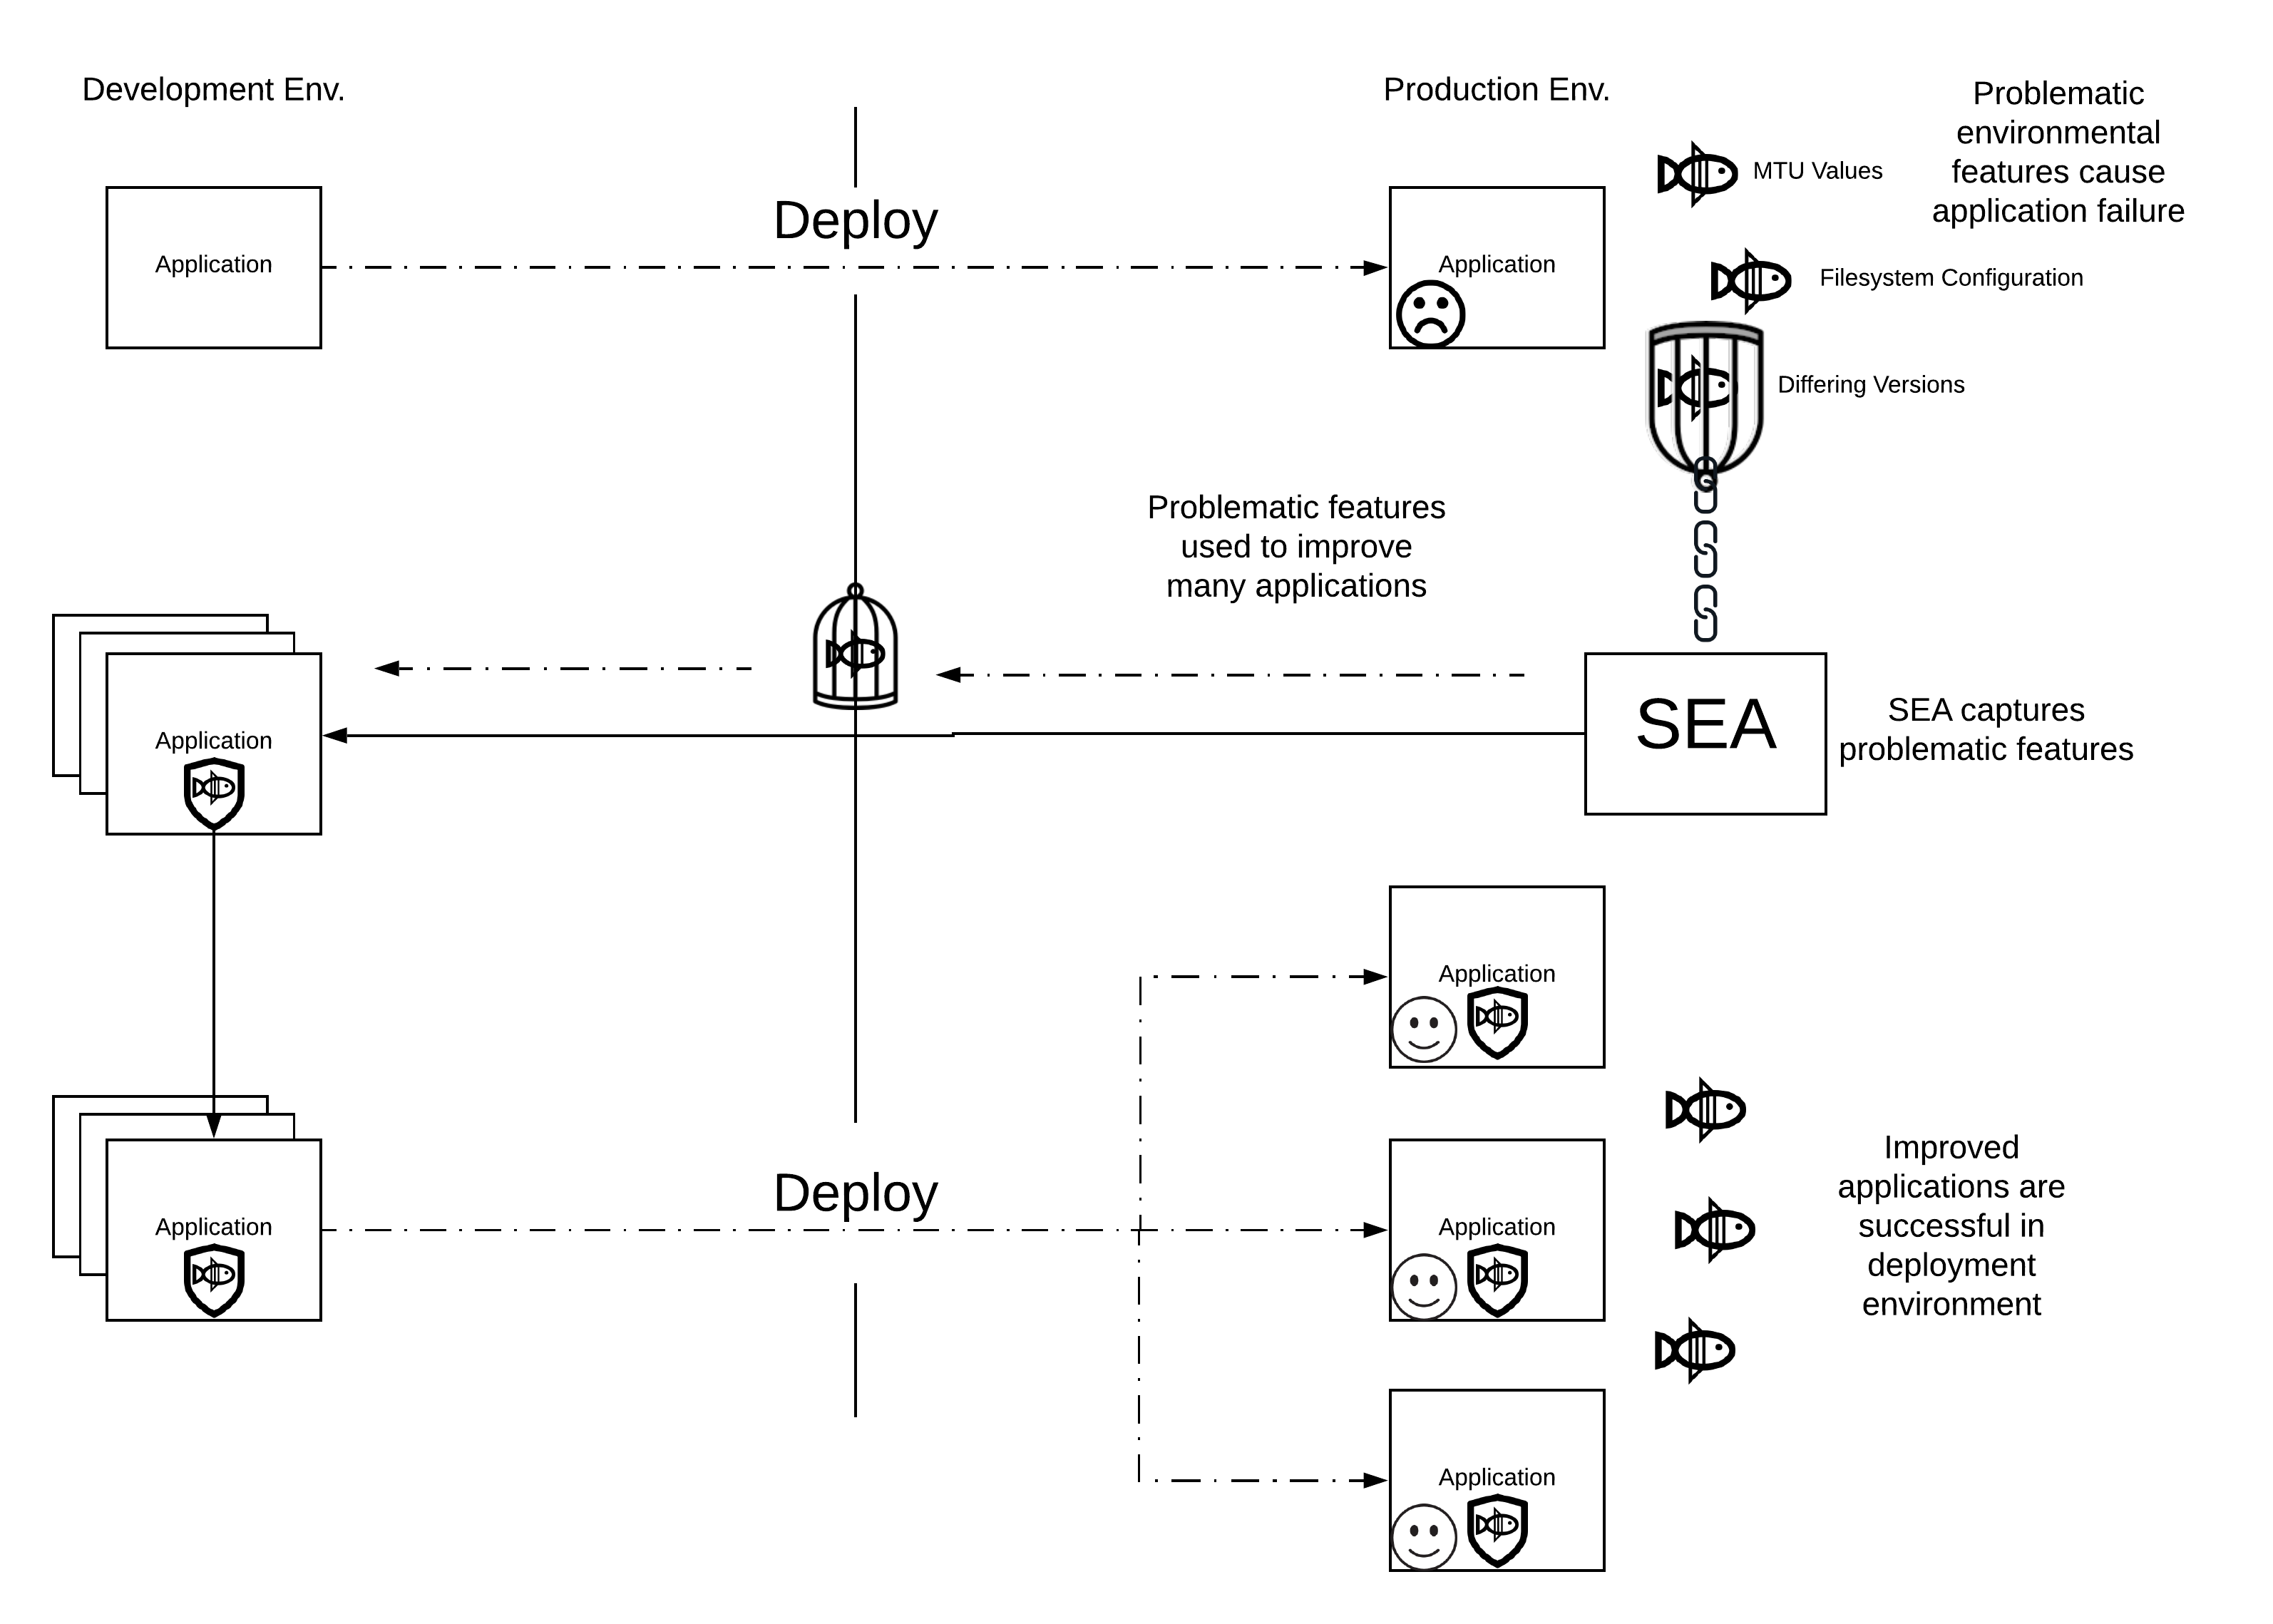
\includegraphics[scale=.37]{images/approach}}
  \caption{Diagram illustrating CrashSimulator's approach}
  \label{figure:approach}
\end{figure}

As mentioned earlier,
the Results Based Simulation (RBS) technique
offers a reliable way to identify bugs
that could arise from interaction with a given environment.
In this section,
we will break down the elements of the technique,
and then introduce a tool called CrashSimulator,
which we built as a concrete implementation of RBS.
We also describe a second technology
called Process Set Cloning
that evolved during our work on CrashSimulator.


\subsection{Stepping through RBS}

The first step in implementing RBS
is selecting an anomaly or anomalies
against which you wish to test applications.
Anomalies can be collected
by examining failures of other applications
in a target deployment environment,
exploring public bug trackers,
or by using tools that can identify
potentially problematic environmental conditions~\cite{Zhuang_NSDI_2014,
rasley2015detecting}.
Identifying anomalies through bugs posted on public trackers
is ideal when determining
whether or not an application
is vulnerable to a widely publicized bug.
The chosen anomalies are then examined
in order to determine how they cause an application's communications
with its environment
to differ from a normal execution.
Once they have been teased out,
these differences can be represented
as a set of modifications
that must be made to an application's communications
in order to simulate the chosen anomaly or anomalies.
As an example,
consider an anomalous environment
where access to a required file is denied because of
the environment's configured file permissions.
This anomaly presents as attempts to access the file,
such as calls to {\tt fread()},
the {\tt read()} system call,
or other file access mechanisms,
returning an error stating that access to the file is denied.
The ``modification'' required to simulate this anomaly
is to change the results of similar accesses
in a test execution
to return ``access denied.''

The second step
is identifying
a way to monitor an application's communication
with its environment,
by redirecting function calls,
observing memory access,
monitoring network activity,
intercepting system calls,
or some other similar means.
These opportunities are identified by looking at the parameters,
return values,
and orderings,
of an application's communications
that indicate
it is an appropriate time to simulate an anomaly.
Monitoring an application's communications
in this fashion
has the added benefit
of allowing us to find obvious situations
where an application will fail
to handle certain environmental features.
This is possible because an application's failure
to carry out required operations is visible as it interacts
with its environment.
Consider an application that fails to check whether or not
a file already exists
before destructively opening it and writing to it.
The absence of this check
is problematic in environments where the file already exists
as it will be blindly overwritten.
Because it is obvious from the sequence of communications
the application makes when writing to the file
that this check has been neglected,
no simulation is required to identify the presence of a bug.


Included with CrashSimulator is a corpus of environmental anomalies
that we found to be problematic for real world
applications.
From a user's perspective, using CrashSimulator boils down to selecting one
of the supplied anomalies to test an application against and allowing the
tool to take over.  Behind the scenes,
a four-step operation is used to identify bugs resulting from
the chosen anomaly.
These steps, illustrated in Figure~\ref{figure:approach} are as follows.
First, CrashSimulator records the application being tested.  Next, it
modifies this recording so that the chosen anomaly is present.
Finally, It then replays this
modified recording, exposing the application to the chosen anomaly.

\subsection{Trace Recording and Anomaly Injection}

Before testing can begin
CrashSimulator generates recording of the application to be
tested as it executes in an environment where the chosen anomaly is not
present.  This recording acts both as a medium into which anomalies can be
injected and a log of the application's behavior under normal
conditions.  Once this recording is complete CrashSimulator runs a script,
known as a mutator, associated with the chosen anomaly.
This script is responsible for identifying
the points in the recording
where the anomaly can be injected and modifying
the recording such that the anomaly is present.

Once this mutated recording has been generated, CrashSimulator replays the
application using this recording.
Because replaying the
recording faithfully follows the described system call behavior, the
application is exposed to the injected
anomalous conditions.  For
example, suppose an anomaly causes a call to {\tt read()} to fail with
return value of -1 and {\tt errno} set to {\tt EINVAL}.  Exposing an
application to this situation only requires modifying the recording,
such that this read call reflects the above values.

We refer to this process as {\tt Result Based Simulation} and it hinges on
on the idea that environmental anomalies will be present in the results of
the procedure calls an application makes that are influenced by the
applications environment.
This technique could be carried out several different levels
of execution.  For example, the results of calls to functions in a
platform's {\tt libc} library could be intercepted and modified to reflect
environmental differences.  At a higher level, virtual machines like the
{\tt JVM} could be adapted to allow the results and side effects of calls
to be interposed upon in a similar fashion.
For CrashSimulator's purposes we chose to influence
the results and side effects of system calls in order to simulate
unusual environment.  Operating at this level provides a few key
advantages.  First, there is already robust tooling in the Linux kernel
that allows for the interception and modification of system call results
and side effects.  Additionally, Linux system call semantics are well
defined which simplifies implementation.  Finally, operating at this level
allows CrashSimulator to test applications written any language that can
execute Linux system calls.

\subsection{Analyzing an Execution}

After an application has been exposed to an anomaly CrashSimulator must
make a determination about whether the application may be responding to it.
This determination comes down to whether or not
the application alters its
system call behavior.  When an anomalous
behavior is injected into a replay execution,
it is expected that the application under
test will deal with it in some way.  For example, applications can
be expected to behave differently when the structure returned by a call to
{\tt stat()} indicates the target file is a block device,
rather than a regular
file.  CrashSimulator bases its assessment on the assumption that the way
an
application deals with the anomaly will yield
different program paths (and therefore different system calls) than
those
executed when the original system call trace was recorded.
If the application
does not alter its behavior, it has not
correctly handled this flaw --- a failing result.  Alternatively, if the
application does deviate, it is likely that the application is taking some
action to handle the injected condition --- an indication of possibly
correct behavior.

This approach is often sufficient to classify application behavior.  As
with traditional tests, CrashSimulator does not tell us that an application
is bug free in a given situation; instead, it asserts that an application
has incorrectly handled a given situation.  In our experience, actually
exposing applications to anomalies CrashSimulator reported as unhandled
did result
in bugs ranging from simple hangs to more dramatic crashes that
had the side effect of consuming all available resources or filling
available disk space with garbage.
